前章では、電気信号が届いた際に問題となる「同期」について記した。では、実際に情報を電気信号に乗せ、送るにはどういう方法を取ればよいだろうか。本章および次章ではまさしく通信の本丸と言える信号の伝送について説明する。本章では伝送方式を概観し、その基本となる伝送方式のベースバンド伝送方式について解説を行う。

\section{信号伝送方式}

コンピュータに記録されたデータはbitにより構成されている。この構成する0と1を意味するように電圧の高低を二元状態に当ててやれば、電圧が情報を表していると言える。この電圧の変化はパルス\footnote{短時間に急峻な変化をする信号のこと。また、通信等の分野においては矩形的な変化をする波もパルスと呼ぶ。}であり、そのまま電圧変化として送信することもできる。このように、信号を変換した波をそのままに伝送する方式を\textbf{ベースバンド伝送}\index{べーすばんどでんそう@ベースバンド伝送}または\textbf{基底帯域伝送}\index{きていたいいきでんそう@基底帯域伝送|see{ベースバンド伝送}}と呼ぶ。

一方、波をそのまま送るのではなく、他の\textbf{搬送波}\index{はんそうは@搬送波}(\textbf{キャリア}\index{きゃりあ@キャリア|see{搬送波}}とも)に載せて信号を送る手法もある。この手法を\textbf{ブロードバンド伝送}\index{ぶろーどばんどでんそう@ブロードバンド伝送}または\textbf{帯域伝送}\index{たいいきでんそう@帯域伝送|see{ブロードバンド伝送}}と呼ぶ。ベースバンドよりも装置などが複雑になるが、搬送波に載せて信号を送ることによる様々なメリットが必要となることも多いためこちらの方法が取られるものも多い。

本章では、ベースバンド伝送方式の仕組みと利点について見ていく。帯域伝送方式については次章で取り扱う。

\section{ベースバンド伝送方式}
ベースバンド伝送は、古くから有線通信に使われてきており、現代でもLANの通信や固定電話の一部などで利用されている。古くから使われる理由は、単純な方式で実現が容易であるからと言える。

\subsection{ベースバンド伝送方式の要件}
ベースバンド伝送に必要とされる要件は大きく次の3点である。

\begin{itembox}[l]{ベースバンド伝送方式の要件}
\begin{itemize}
\item 連続性の抑圧:0or1が連続するとタイミング抽出がしにくく(=同期が難しく)なるため、連続しすぎないこと。
\item パワースペクトルの集中性:電圧の変化があまり頻繁(高周波)であると、伝送路によって伝えられないことが起こるため、電圧の周波数がある一定の幅に集中しているのが望ましい。
\item 直流平衡:直流遮断特性(機械の保全等のため直流電圧を通さない特性)による遮断の影響が少ないこと。
\end{itemize}
\end{itembox}

これらの要件のため、後に上げるような様々なベースバンド伝送方式が有り、回路や機械の特性に応じて利用方式が変わる。

\subsection{ベースバンド伝送方式の特徴}
ベースバンド伝送は単なる電気の伝送であるため、長距離でなければ比較的単純に装置を準備できる。このように、回路規模が小さいのがベースバンド伝送方式の特徴である。

一方で、一度に一つの信号しか送れない、雑音に弱い、無線通信では実現が難しいなどの難点もある。特に、最初の「1つの信号しか送れない」点は実際の通信において大きな欠点となる。帯域伝送方式を利用することが多いのはこの難点の解消のためであるが、逆に小規模な伝送では不要な(気にしなくてよい)問題であるためにベースバンド伝送も現役で使われていると言える。

\subsection{ベースバンド伝送方式の分類}
ベースバンド伝送方式は、どのような電圧状態を1/0に対応させるかによって分類が分かれる。以下、その各方式について記述していく。尚、通常は電圧0の状態と電圧$E$ないし$-E$の状態を用いることとなるが、以下は便宜のため0と1/-1を使っているとして記述する。

\subsubsection{RZとNRZ}
あるbitを表す単位時間の電圧のうち半分を電圧0に当てる方式を\textbf{RZ方式}\index{RZほうしき@RZ方式}(Return to Zero方式)と呼ぶ。対して特段そのような措置を取らない手法もあり、この場合は\textbf{NRZ方式}\index{NRZほうしき@NRZ方式}(Non Return to Zero方式)と呼ぶ。RZ方式はビットパルスの半分が0となるのでビット同期に都合が良い。	対してNRZ方式は電圧の変化が少なくなるため、電圧の変化が高周波でなくなるという利点がある。
  

\subsubsection{両極方式と単極方式}
先のRZ方式/NRZ方式に加え、電圧変化にどの幅を使うかにより、\textbf{両極方式}\index{りょうきょくほうしき@両極方式}と\textbf{単極方式}\index{たんきょくほうしき@単極方式}の2種類の方式がある。前者は正極(電圧+1)と負極(電圧-1)を各々1/0に割り当てて利用する。後者の単極方式では正極または負極の一方と電圧0の状態を1/0に割り当てる。

図\ref{fig5_1}に、単極・両極のRZ/NRZ方式の例を示す。
\begin{figure}[htbp]
\centering
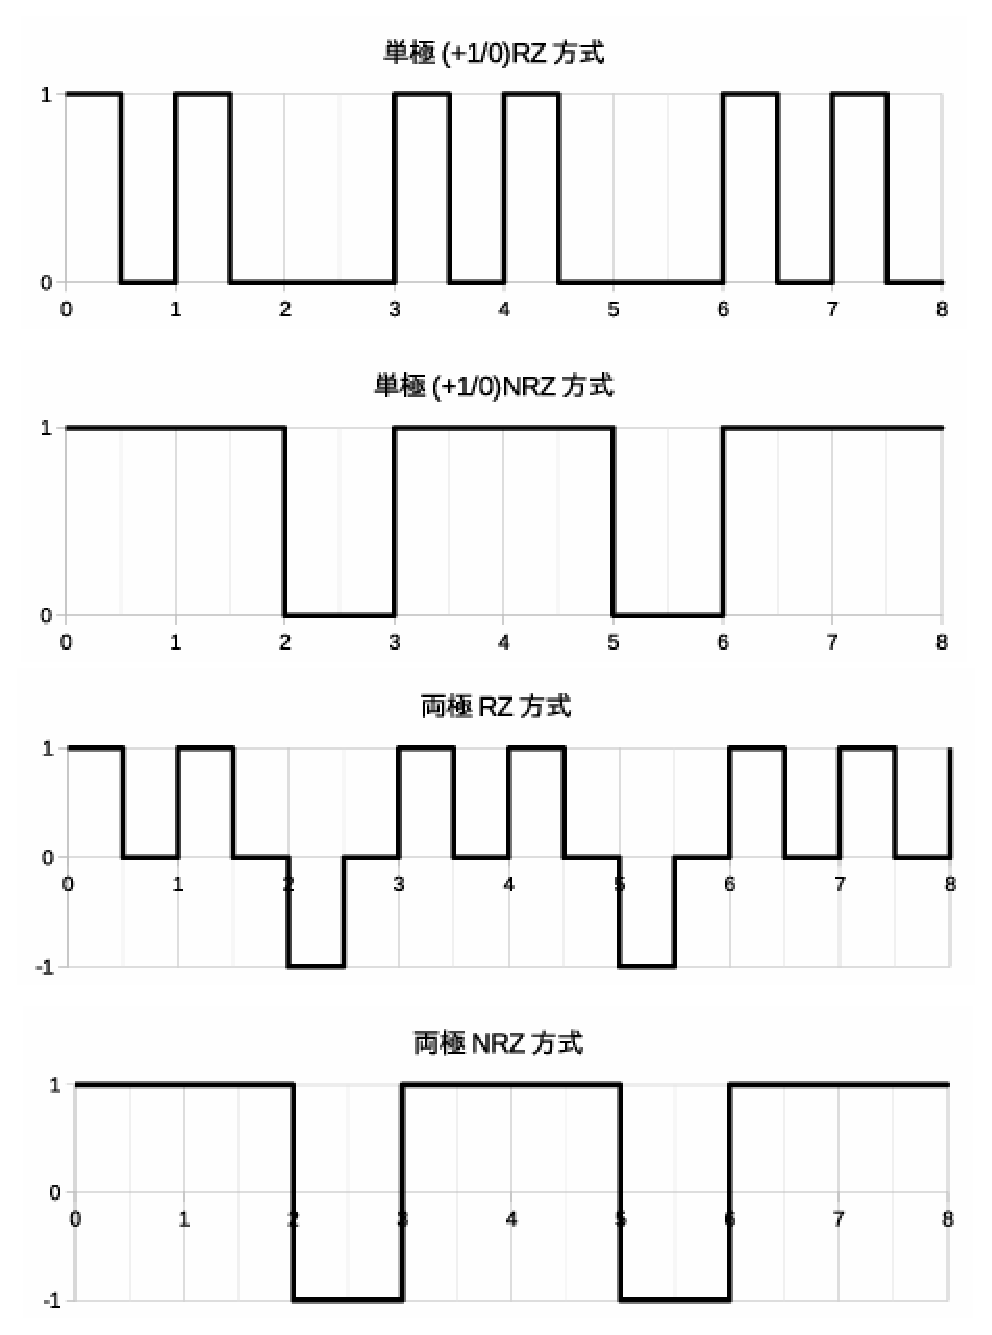
\includegraphics[width=0.8\linewidth,keepaspectratio]{fig/fig5_1.eps}
\caption{単極・両極のRZ・NRZ方式における符号語11011011の電圧変化。横軸の数値はビットの単位時間を示す。}
\label{fig5_1}
\end{figure}

\subsubsection{バイポーラ方式}  
\textbf{バイポーラ方式}\index{ばいぽーらほうしき@バイポーラ方式}(bipolar system)では、正極/負極をともにビット1に当て、電圧0を0に割り当てる。つまり、電圧の絶対値が1/0に対応する。また、1を送り出す場合は「前回1を送ったときと異なる側の極」を使う。つまり、正極を使って1を送った後は(その後にいくつ0があろうとも)次の1は負極を用いて送る。逆もしかりである。この手法では、直流遮断特性の影響を取り除くことができるが、0が連続した場合にビット同期が取り難いという難点もある。

図\ref{fig5_2}に、バイポーラ方式のRZ/NRZ方式の例を示す。
\begin{figure}[htbp]
\centering
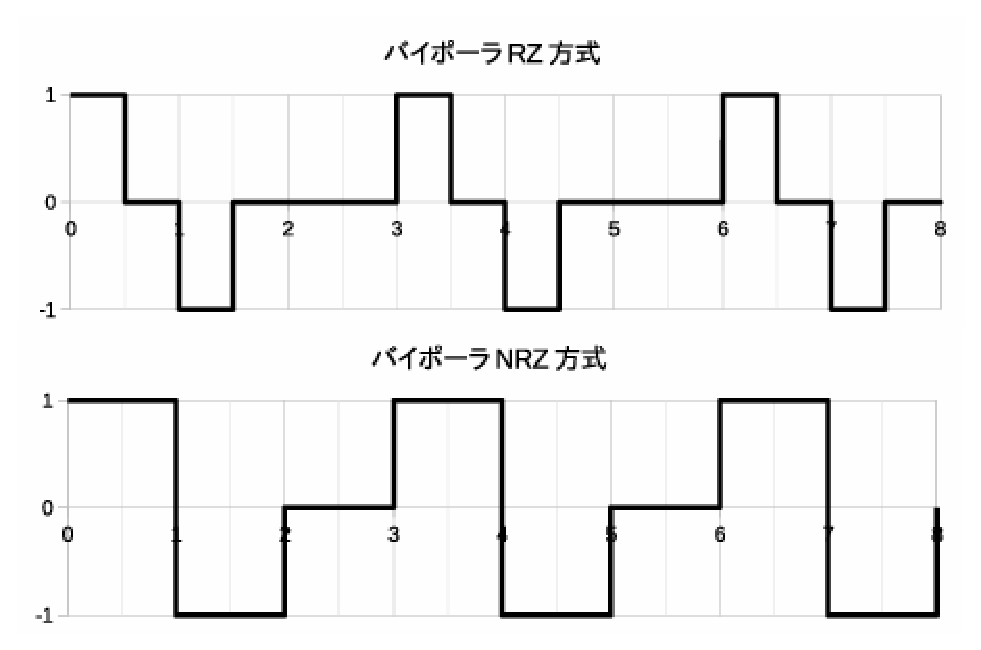
\includegraphics[width=0.8\linewidth,keepaspectratio]{fig/fig5_2.eps}
\caption{バイポーラRZ/NRZ方式における符号語11011011の電圧変化。横軸の数値はビットの単位時間を示す。}
\label{fig5_2}
\end{figure}


\subsubsection{差分方式} 
\textbf{差分方式}\index{さぶんほうしき@差分方式}(differential system) は前の単位時間の電圧から電圧に変化があった場合は1を、なかった場合には0を示す方式である。例えば、ある初期状態の電圧が-1であり、次の単位時間が1、その次の単位時間でも1だったとすると、これは10という符号語になる。

図\ref{fig5_3}に、差分NRZ方式の例を示す(RZ方式では各単位時間後半を0にした図となる)。
\begin{figure}[htbp]
\centering
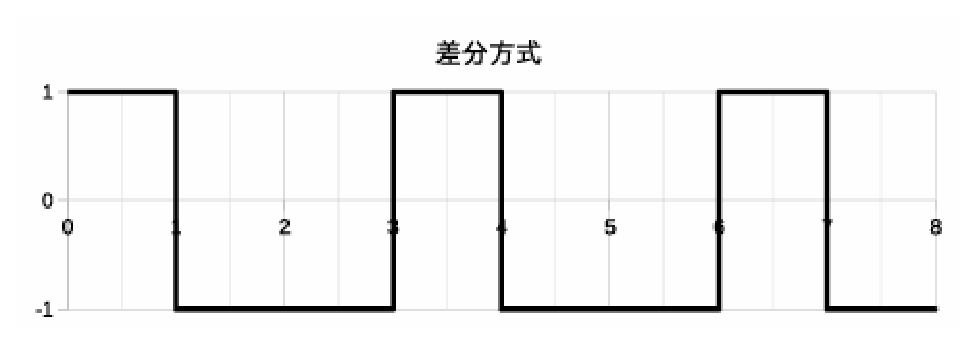
\includegraphics[width=0.8\linewidth,keepaspectratio]{fig/fig5_3.eps}
\caption{差分NRZ方式における符号語11011011の電圧変化。グラフに出ていないが初期状態は-1としている。横軸の数値はビットの単位時間を示す。}
\label{fig5_3}
\end{figure}


\subsubsection{ダイコード方式} 
\textbf{ダイコード方式}\index{だいこーどほうしき@ダイコード方式}(dicode system)では現在のビットが1から0へ変化する場合-1,0から1へ変化する場合1、変化しない場合0の電圧によって表す。初期状態のビットが0であるとして、1の電圧,0の電圧,-1の電圧と続いた場合の符号語は110となる。

図\ref{fig5_4}に、ダイコードNRZ方式の例を示す(RZ方式では各単位時間後半を0にした図となる)。
\begin{figure}[htbp]
\centering
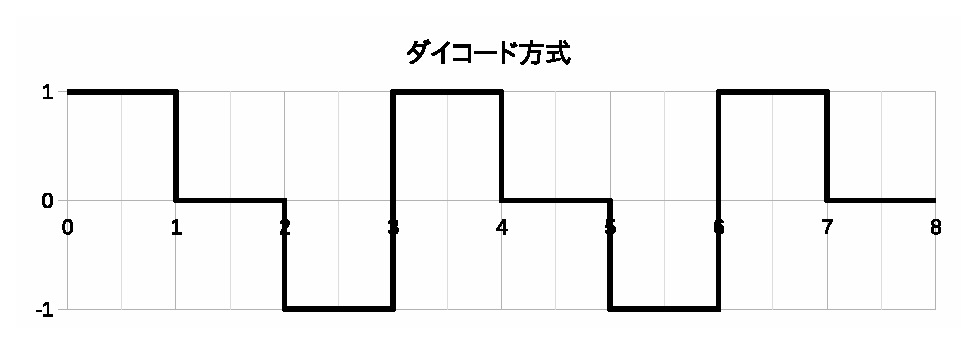
\includegraphics[width=0.8\linewidth,keepaspectratio]{fig/fig5_4.eps}
\caption{ダイコードNRZ方式における符号語11011011の電圧変化。グラフに出ていないが初期状態は0としている。横軸の数値はビットの単位時間を示す。}
\label{fig5_4}
\end{figure}


\subsubsection{マンチェスター/ダイパルス方式}
\textbf{マンチェスター方式}\index{まんちぇすたーほうしき@マンチェスター方式}(Manchester system)あるいは\textbf{ダイパルス方式}\index{だいぱるすほうしき@ダイパルス方式|see{マンチェスター方式}}(dipulse system)は0・1で180度位相の違うパルスを送出するものである。通常、ビットの中心で位相を反転させる(このことから、split-phase符号などとも呼ばれる)。例えば最初-1でスタートしてビットの中心で電圧を1に変えた場合1、その逆に最初1でスタートして後半を-1に変えた場合は0とするのである。位相の反転のおかげでビット同期を取りやすく、後述するEthernet LANで用いられている。

図\ref{fig5_5}に、マンチェスター方式のRZ/NRZ方式の例を示す。
\begin{figure}[htbp]
\centering
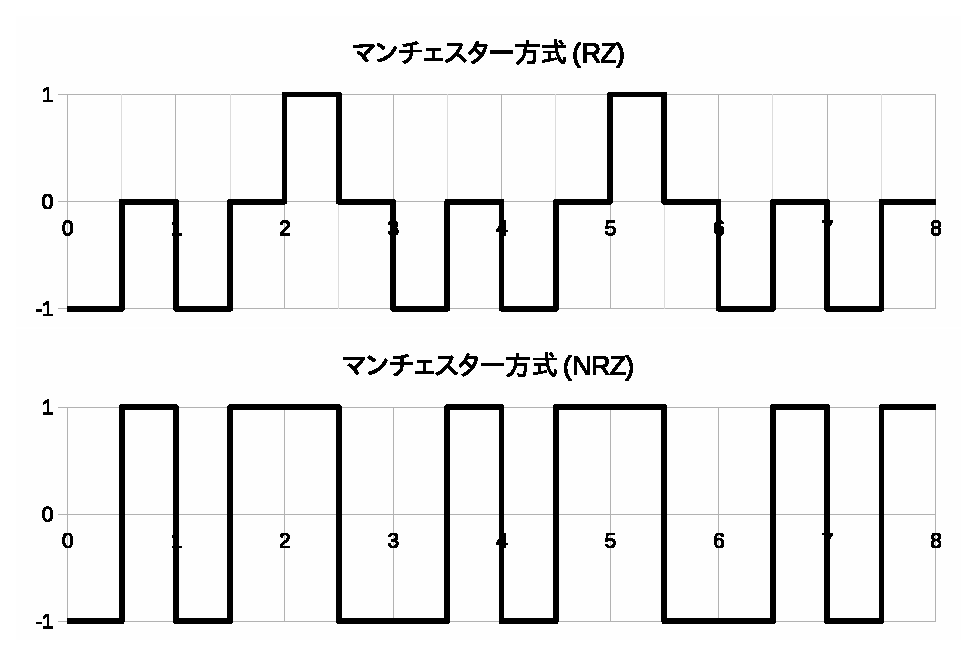
\includegraphics[width=0.8\linewidth,keepaspectratio]{fig/fig5_5.eps}
\caption{マンチェスターRZ/NRZ方式における符号語11011011の電圧変化。横軸の数値はビットの単位時間を示す。}
\label{fig5_5}
\end{figure}
    

\section{伝送速度}
ベースバンド伝送の場合、\textbf{伝送速度}\index{でんそうそくど@伝送速度}は約50kbpsから16Mbpsである。この速度でよく使われる単位"bps"についてここで付章的ながら説明しておく。

bpsはbit/secと書くこともあるが、bit per second(bit毎秒)という単位である。例えば、100bpsは1秒間に100bit=2進数100桁を伝送する速度ということである。似た単位にBpsというのもある。Bを大文字にした場合は一般にByte per second(Byte毎秒)として1秒間に何バイトのデータを伝送するかという単位になる。現在1Byte=8bitであるので、1Bps=8bpsである。

回線速度測定サービスというのがしばしばあるが、これは大きなファイルを用意して、これを送信するのにかかった時間により速度を計算している。300MBのファイルを5分でダウンロードできたとすれば、下りの実効速度\footnote{標榜されている速度ではなく、実際の速度のこと。}は1MBps=8Mbpsとなる。

\subsection{【補足】単位の接頭辞}
\begin{center}
\begin{minipage}[]{0.75\linewidth}
\begin{screen}
\begin{center}
本節は前提知識の補足である。\\
既知の読者におかれては飛ばして次節を読まれたい。
\end{center}
\end{screen}
\end{minipage}
\end{center}

bpsあるいはBps(Byteも含む)単位の接頭辞としては、k(キロ),M(メガ),G(ギガ),T(テラ),P(ペタ)あたりが用いられる。kは$10^3$を示し、以下$10^6,10^9,10^{12},10^{15}$となる。

一方、コンピュータ技術を論ずる場合には、2の累乗が都合が良いため、$10^3=1000$を$2^{10}=1024$に置き換えて用いる場合がある。便宜的にk,M,G,T,Pをそのまま用いる場合もあるが、これを明示する場合にはki(キビ),Mi(メビ),Gi(ギビ),Ti(テビ),Pi(ペビ)という単位(各々$2^{10},2^{20},2^{30},2^{40},2^{50}$)を用いる。

時折、外付けHDDをコンピュータに接続した場合、パッケージ記載の値と容量が異なるように見える場合がある。この原因として、先の$10^3$と$2^{10}$の違いが出てくることがある。例えば1TBのHDDは、$10^{12}$で計算した場合と$2^{40}$で計算すると約100GB,10\%もの違いが出る。

\section*{演習問題}
\begin{problems}
\item 本章内で説明しなかった方式に差動マンチェスタ方式がある。これは、次のようにして定まる。
\begin{itemize}
\item ビットの変わり目で電圧を反対側の極にする(+1なら-1、-1なら+1)。
\item ビットの値が0であれば、1ビット極電圧を維持する。
\item ビットの値が1であれば、ビット中間にてその電圧を反対側の極にする。
\end{itemize}
この差動マンチェスタ方式について、符号語11011011を送る場合、電圧変化はどのようになるか図示せよ。

\item 本章内で出てきた全方式(前問の差動マンチェスタ方式を含む)について、符号語10010011を送る場合の電圧変化を図示せよ。

\item 2000年台前半のソフトウェア公開サイトでは、代表的な速度56kbps(モデム), 64kbps(ISDN), 1Mbps(ADSL), 100Mbps(FTTH)について、ダウンロードにかかる時間が表示されていることがしばしばあった。

ダウンロード対象ファイルのサイズが入力されるとき、先の4回線と自身の好きな速度の1回線でのダウンロード時間を出力するプログラムを作成せよ。ファイルのサイズは小数第2位までの数値と接頭辞(G,M,k,Gi,Mi,ki)及びB(バイト)で入力されるものとする(10.25MBなど。)。なお、入力されるファイルサイズは必ず接頭辞がついてあるものとして良い。

\end{problems}
